The source model used for this test case comprises a simple vertical strike-slip fault using a single magnitude MFD.\\

\noindent Details of the source model are listed below:\\

\noindent
Fault type: Strike slip\\
Fault dip: $90^{\circ}$\\
Fault plane depths: 0--1 km\\
Fault coordinates:\\
South end: $38.1124^{\circ} N$, $122.0450^{\circ} W$\\
North end: $38.1124^{\circ} N$, $121.9550^{\circ} W$\\
Rupture aspect ratio: 1.0\\
Rake angle: $0^{\circ}$\\
Magnitude scaling relationship: PEER MSR\\
Magnitude-frequency distribution:\\
Incremental MFD: $M_{min} = 4.0$; bin width = $1.0$; occurance rate = $1.0$\\

Apart from the different source model, this case is similar to Case~1a, and is only included here as the numbers from this case will be useful in later cases involving a nontrivial source model logic tree with more than branch. The loss curve calculated using the implementation of the calculator in Julia is compared with that produced by OpenQuake in Figure~\ref{fig:lc-ebr-1b}.

\begin{figure}[htbp]
\centering
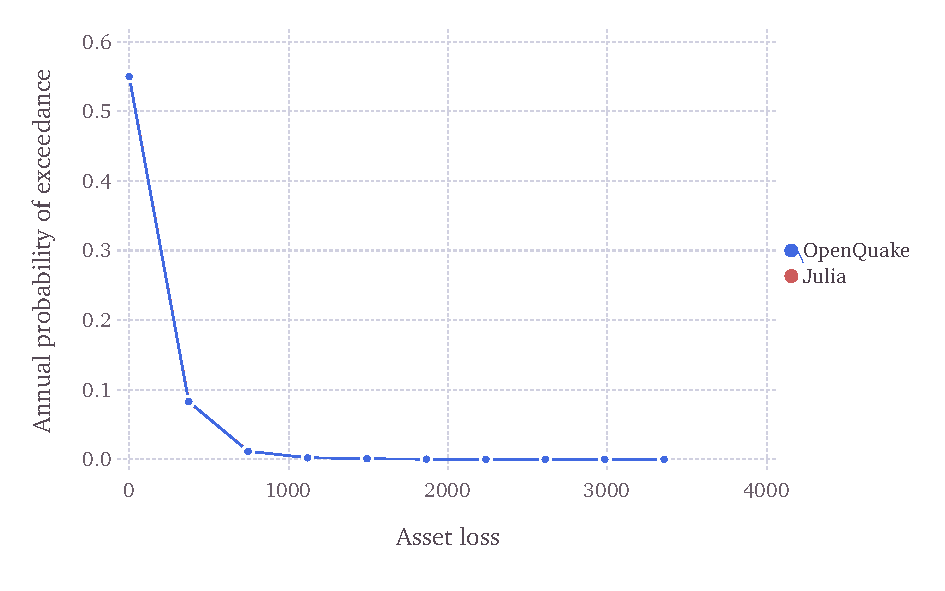
\includegraphics[width=12cm]{qareport/figures/fig-lc-ebr-1b}
\caption{Loss curve comparison for event based risk test case 1b}
\label{fig:lc-ebr-1b}
\end{figure}

The area under the annual loss exceedance curve gives the average annual loss.